%% Adapted from GaTech CS 7545 Machine Learning Theory given by Prof. Jacob Abernathy Fall 2018. Original latex file: https://github.com/mltheory/CS7545/blob/master/scribe/CS7545scribe_template.tex 



%%%%%PLEASE CONSIDER CORRECTIONS AT PLACES INDICATED%%%%%%%%
\documentclass{article}
%%%%%Packages Used, add more if necessary%%%%
\usepackage{amsmath,amsfonts,amssymb,graphicx,fullpage, float}
\setlength{\topmargin}{-0.6 in}
\setlength{\textheight}{8.5 in}
\setlength{\headsep}{0.75 in}
\usepackage{mdframed}
\usepackage{multicol}
\usepackage{microtype}
\usepackage{mdframed}
\usepackage{multicol}
\usepackage{microtype}
\usepackage{listings}
\usepackage{graphicx}
\usepackage{float, hyperref} 


%%%%% NO NEED TO EDIT THIS PREAMBLE %%%%%%%%
%%% PREAMBLE %%%
\newcounter{lecnum}
\renewcommand{\thepage}{\thelecnum-\arabic{page}}
\renewcommand{\thesection}{\thelecnum.\arabic{section}}
\renewcommand{\theequation}{\thelecnum.\arabic{equation}}
\renewcommand{\thefigure}{\thelecnum.\arabic{figure}}
\renewcommand{\thetable}{\thelecnum.\arabic{table}}
\newcommand{\lecture}[4]{
   \pagestyle{myheadings}
   \thispagestyle{plain}
   \newpage
   \setcounter{lecnum}{#1}
   \setcounter{page}{1}
   \noindent
   \begin{center}
   \framebox{
      \vbox{\vspace{2mm}
      
      \hbox to 6.28in { 
      {\bf ECE 4252/6252 (FunML) Fundamentals of Machine Learning \hfill 2021--2028} }
      
      \vspace{2mm}
      \hbox to 6.28in { 
      {Courses developed by Professor Ghassan AlRegib 
      (\href{https://alregib.ece.gatech.edu/}{alregib.ece.gatech.edu}) 
      \hfill For inquiries: \href{mailto:alregib@gatech.edu}{alregib@gatech.edu}} }
      
      \vspace{3mm}
      \hbox to 6.28in { {\Large \hfill Lecture #1: #2 \hfill} }
      
      \vspace{2mm}
      \hbox to 6.28in { {\it Co-Instructors: #3 \hfill #4} }
      
      \vspace{2mm}}
   }
   \end{center}

   % -------- PEOPLE OUTSIDE BOX --------
   \vspace{2mm}
   \noindent{\bf Contributors:} Dr. Ahmad Mustafa, Dr. Motaz Alfarraj, Dr. Ashraf Alattar, Dr. Chen Zhou

   \vspace{1mm}
   \noindent{\bf Teaching Assistants} with remarkable contributions include: Kuo-Wei Lai, Wuyang Du, Shiva Mahato, Michael Zhou, Ninghan Zhong

   \markboth{Lecture #1: #2}{Lecture #1: #2}

   \vspace{2mm}
\noindent {\bf Disclaimer}: 
{All content of these notes are part of this course at Georgia Tech. Any re-use or distribution is not permitted without pre-approved permission. All these notes belong to, created by, and copyrighted for Ghassan AlRegib and Mohit Prabhushankar, Georgia Tech, 2021--2028.}

\vspace{2mm}
\noindent {\bf License}: 
{These lecture notes are licensed under the 
\href{https://creativecommons.org/licenses/by-nc-sa/4.0/}{Creative Commons Attribution-NonCommercial-ShareAlike 4.0 International License}.}

   \vspace{2mm}
   \noindent {\bf Errata}: 
   {\it Please submit any errata you find using the following form: 
   \href{https://forms.office.com/r/fbg9dMWPgY}{Errata Form for FunML Textbook} 
   or visit: \url{https://forms.office.com/r/fbg9dMWPgY}}

   \vspace*{4mm}
}
\renewcommand{\cite}[1]{[#1]}
\def\beginrefs{\begin{list}
        {[\arabic{equation}]}{\usecounter{equation}
         \setlength{\leftmargin}{2.0truecm}\setlength{\labelsep}{0.4truecm}%
         \setlength{\labelwidth}{1.6truecm}}}
\def\endrefs{\end{list}}
\def\bibentry#1{\item[\hbox{[#1]}]}

\newcommand{\challenge}[2]{\noindent \textbf{(Challenge Problem)} \emph{#1}: #2 }

\newcommand{\exercise}[1]{\noindent \textbf{(Exercise)} #1 }

\newcommand{\fig}[3]{
			\vspace{#2}
			\begin{center}
			Figure \thelecnum.#1:~#3
			\end{center}
	}
%%% END_OF_PREAMBLE %%%


	
%%%%You may add more \newtheorem if necessary%%%%%%
\newtheorem{theorem}{Theorem}[lecnum]
\newtheorem{lemma}[theorem]{Lemma}
\newtheorem{proposition}[theorem]{Proposition}
\newtheorem{claim}[theorem]{Claim}
\newtheorem{corollary}[theorem]{Corollary}
\newtheorem{definition}[theorem]{Definition}
\newenvironment{proof}{{\bf Proof:}}{\hfill\rule{2mm}{2mm}}


\newcommand{\dom}{\mathrm{dom}}
\begin{document}

%%%%%CHANGE HERE%%%%%%%
%%%%%\section{title of the section} similarly with the rest \section{} or \subsection{} or \subsubsection{} etc


%%%%%CHANGE HERE%%%%%%%%%
%%%%%\lecture{the ordinal number of the lecture}{lecture title}{Jacob Abernethy}{scriber's name}%%%%%%%%
\lecture{22}{Explainability in Neural Networks}{Ghassan AlRegib and Mohit Prabhushankar}{}

%%%%%CHANGE HERE%%%%%%%
%%%%%\section{title of the section} similarly with the rest \section{} or \subsection{} or \subsubsection{} etc

\section{Lecture Objectives}

In this lecture, we introduce visualization-based techniques for interpreting
deep neural networks. We examine why modern models are often difficult to
interpret and how visualization methods can help translate internal
representations into human-understandable insights. We study perturbation-based
and gradient-based saliency methods, including Vanilla Backpropagation,
Deconvnet, and Guided Backpropagation, and discuss how these techniques reveal
which input regions influence a model’s prediction. We then introduce Grad-CAM,
a method that produces class-discriminative and spatially meaningful
explanations by leveraging gradients in the final convolutional layer. Together,
these tools provide a foundation for understanding how neural networks make
visual decisions.


% \section{Recap} 
% %%%%%Use itemize to layout bullet points that are not numbered%%%%%

% In the previous lecture, we dived into explainability in machine learning, particularly within neural networks, covering methods like Grad-CAM and saliency maps, and evaluating these techniques through both human-centered and application-based approaches to enhance understanding and trust in ML models.




\section{Explainability}

\subsection{Definition}
\textbf{Explainability} refers to the ability of a machine learning model to clearly describe, justify, or provide human-understandable reasons for its predictions or decisions. In other words, an explainable model allows a human user to understand \emph{why} a particular output was produced for a given input.

Explainability helps bridge the gap between complex mathematical models and human interpretation by translating internal model behavior into meaningful insights that can be interpreted, trusted, and verified.

\subsection{Why do we choose explainability}
Explainability in deep learning systems is crucial for building \textbf{trust, transparency, and accountability}. Modern neural networks often achieve high predictive accuracy, but they typically operate as \emph{black-box models}, meaning their internal reasoning is not directly interpretable.

Explainable models are particularly valuable in high-stakes domains such as healthcare, where they assist doctors in diagnosis and treatment decisions; seismic interpretation, where they help experts label and analyze geological data; and autonomous systems, where they increase safety and reliability by clarifying why specific actions are taken.

Without explainability, models simply map inputs to outputs (e.g., class scores) without providing insight into the reasoning behind those predictions. This lack of transparency limits adoption, debugging, and responsible deployment of machine learning systems.


\subsection{Explainability in CNNs}
We begin by examining a classical convolutional neural network (CNN) architecture, AlexNet. 
Understanding the structure of CNNs is important because many explainability techniques 
analyze how information flows through these layers and which layers contribute most 
to the final prediction.

\paragraph{A brief look at AlexNet}

\begin{figure}[H]
    \centering
    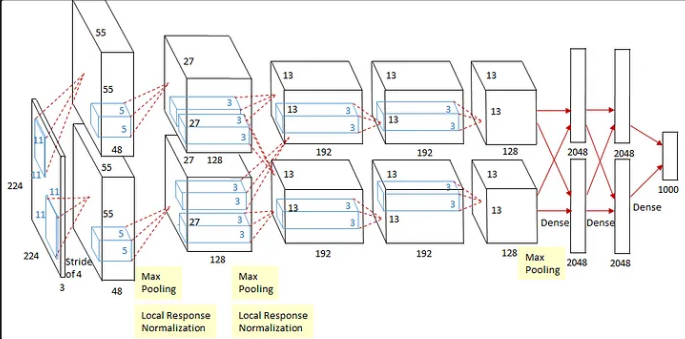
\includegraphics[width=1.0\linewidth]{img/lecture22/01.png}
    \caption{Figure 22.1: Different layers in a CNN}
    \label{fig:Architecture of AlexNet}
\end{figure}

\paragraph{}
AlexNet contains eight learnable layers:

\begin{itemize}
    \item \textbf{Input:} $227\times227\times3$ images.  
    (The paper sometimes mentions $224\times224\times3$; in practice this size is padded to 227 before the first convolution.)

    \item \textbf{1st Convolutional Layer:} Two groups of 48 kernels of size $11\times11\times3$ (stride 4, padding 0).  
    Output: $55\times55\times48$ feature maps per group.  
    Followed by $3\times3$ overlapping max pooling (stride 2) → $27\times27\times48$.  
    Then Local Response Normalization (LRN).

    \item \textbf{2nd Convolutional Layer:} Two groups of 128 kernels of size $5\times5\times48$ (stride 1, padding 2).  
    Output: $27\times27\times128$.  
    Followed by $3\times3$ overlapping max pooling → $13\times13\times128$.  
    Then Local Response Normalization.

    \item \textbf{3rd Convolutional Layer:} Two groups of 192 kernels of size $3\times3\times256$ (stride 1, padding 1).  
    Output: $13\times13\times192$.

    \item \textbf{4th Convolutional Layer:} Two groups of 192 kernels of size $3\times3\times192$ (stride 1, padding 1).  
    Output: $13\times13\times192$.

    \item \textbf{5th Convolutional Layer:} 256 kernels of size $3\times3\times192$ (stride 1, padding 1).  
    Output: $13\times13\times256$.  
    Followed by $3\times3$ overlapping max pooling → $6\times6\times256$.

    \item \textbf{6th Fully Connected Layer:} 4096 neurons.
    \item \textbf{7th Fully Connected Layer:} 4096 neurons.
    \item \textbf{8th Fully Connected Layer:} 1000 output neurons (ImageNet classes).  
    Softmax is used for classification.
\end{itemize}

\textbf{Key takeaway:} AlexNet contains approximately \textbf{60 million parameters}, 
highlighting the complexity of modern CNNs and motivating the need for explainability methods.

\section{Visualizing CNNs}

In convolutional neural networks (CNNs), filters can be viewed as learnable weight tensors that detect specific visual patterns from input images. Each filter spans the full depth of the input volume (e.g., 3 channels for RGB images) and produces an activation map indicating where that pattern is detected.

Visualizing these filters helps us understand \emph{what types of features} the network learns at different layers, which is an important step toward explainability.

\subsection{Visualizing Filters in First Layers}

\subsubsection{AlexNet}

\begin{figure}[H]
    \centering
    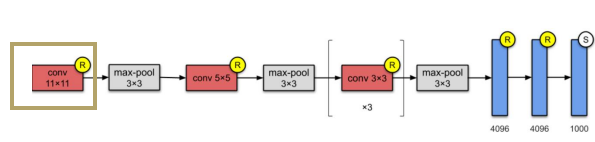
\includegraphics[width=1.0\linewidth]{img/lecture22/AlexNet.png}
    \caption{Figure 22.2: The sequence of convolutional layers of AlexNet}
    \label{fig:The sequence of convolutional layers of AlexNet}
\end{figure}

\begin{itemize}
    \item 64 filters in the first convolutional layer.
    \item Filter size: $11 \times 11 \times 3$ (visualized as RGB images).
    \item These filters typically detect low-level features such as oriented edges, color blobs, textures, and simple patterns.
\end{itemize}

\subsubsection{ResNet}

\begin{figure}[H]
    \centering
    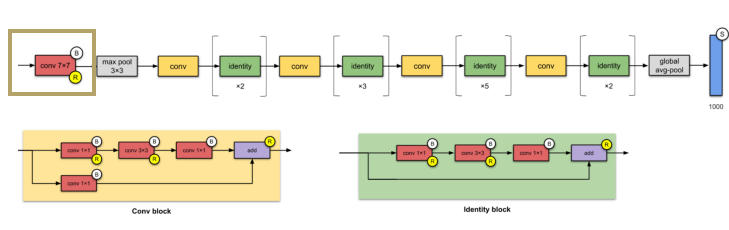
\includegraphics[width=1.0\linewidth]{img/lecture22/ResNet.png}
    \caption{Figure 22.3: The sequence of convolutional layers of ResNet}
    \label{fig:The sequence of convolutional layers of ResNet}
\end{figure}

\begin{itemize}
    \item Uses deeper architectures with identity shortcuts and convolutional blocks to enable training of very deep networks.
    \item First-layer filter size: $7 \times 7 \times 3$ (visualized as RGB images).
    \item 64 filters in the first convolutional layer.
\end{itemize}

\subsubsection{Summary}

Despite architectural differences between AlexNet and ResNet, the filters learned in the first convolutional layers tend to capture very similar low-level visual patterns. These commonly include edge detectors, color transitions, and simple textures. 

This consistency across architectures suggests that early layers learn generic visual primitives, while deeper layers progressively build more complex and class-specific representations.


\subsection{Visualizing Filters in Intermediate Layers}

As we move deeper into a CNN, the learned representations become increasingly abstract and harder to interpret directly. While first-layer filters often resemble simple edge or color detectors, intermediate layers combine these primitive features into more complex and semantically meaningful patterns.

\subsubsection{Layer-specific Details}

\begin{figure}[H]
    \centering
    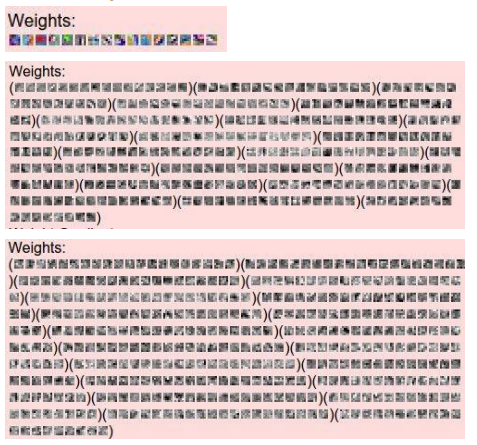
\includegraphics[width=0.5\linewidth]{img/lecture22/layers.png}
    \caption{Figure 22.4: Layer-specific Outputs}
    \label{fig:Layer-specific Outputs}
\end{figure}

In the initial layers (e.g., Conv1), weights can be visualized as RGB images and are relatively interpretable, capturing basic structures such as edges, corners, and textures. In contrast, higher layers (e.g., Conv2 and Conv3) produce weights that appear as more abstract grayscale patterns. These filters represent increasingly complex combinations of lower-level features, making them less interpretable in raw form but more powerful in representation.

\subsubsection{Activation Specificity in Conv5 Layer}

Deeper convolutional layers begin to respond to \textbf{object parts} and higher-level semantic concepts rather than simple edges. For example, the fifth convolutional layer (Conv5) in networks such as AlexNet is particularly sensitive to specific object components, such as wheels. This selectivity is visualized through activation maps, which highlight spatial regions where a filter responds most strongly. These activation maps reveal which parts of the image contribute most to the network’s internal representation and ultimately influence the final prediction.

\begin{figure}[H]
    \centering
    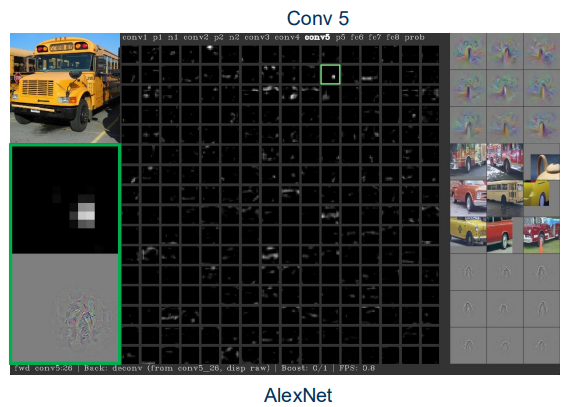
\includegraphics[width=0.6\linewidth]{img/lecture22/conv5.png}
    \caption{Figure 22.5: Conv5 of AlexNet}
    \label{fig:Conv5 of AlexNet}
\end{figure}

\subsection{Maximally Activating Patches}

Beyond visualizing intermediate activations, we can analyze which specific regions of input images cause the strongest responses in individual neurons. \textbf{Maximally activating patches} refer to image regions that trigger the highest activation values for a particular filter within a network. By identifying these regions, we gain insight into what visual patterns a neuron is most sensitive to and what semantic features it has learned to detect.

\subsubsection{Procedure for Obtaining Maximally Activating Patches}

To obtain maximally activating patches, we first select a specific layer and channel (for example, channel 17 in the Conv5 layer). We then pass a large collection of images through the network and record the activation values for that selected channel. Finally, we identify and extract the image regions corresponding to the highest activation values. Visualizing these patches reveals which patterns most strongly excite that neuron.

\subsubsection{Characteristics of Maximally Activating Patches}

Maximally activating patches often display consistent visual structures across different images. For instance, a particular neuron may respond strongly to faces, text, wheels, or other object parts. When visualized row-by-row (each row corresponding to a specific neuron), we typically observe that each neuron specializes in detecting a distinct category of visual patterns. This specialization highlights how deeper CNN layers develop structured and semantically meaningful feature representations.


\subsection{Visualizing Last Layer Activations}

The last layer activations of a CNN are high-dimensional feature vectors (e.g., 4096-dimensional in AlexNet) extracted just before the final classifier. These embeddings summarize the entire input image rather than localized patches, capturing the most abstract and semantically meaningful information learned by the network. Analyzing these representations helps us understand how the model organizes images in its learned feature space.

\subsubsection{Purpose of Last Layer Visualizations}

Images that produce similar last layer activations can be grouped together in the feature space. This similarity indicates that the network perceives them as sharing common semantic characteristics, even if their pixel-level appearance differs. Such grouping is useful for tasks like image retrieval, clustering, and measuring content similarity.

By examining these embeddings, we can also explore how different inputs activate the network in comparable ways, revealing which patterns or concepts the CNN considers related.

\subsubsection{Operational Methodology}

To visualize last layer activations, a large set of images is first passed through the network to extract their final-layer feature vectors. These embeddings are then analyzed—typically by grouping similar vectors or applying dimensionality reduction—to display images that occupy nearby positions in the learned feature space. This process provides a macro-level view of the network’s internal representation structure.

\subsection{Visualizing Last Layer Activations via Dimensionality Reduction}

\subsubsection{Last Layer Embedding}

The last layer embedding is a high-dimensional feature vector (e.g., 4096 dimensions in AlexNet) extracted just before the final classification layer. This vector summarizes the most important features of the image that the network uses to make its prediction. However, because humans cannot directly visualize thousands of dimensions, we require techniques that project these embeddings into lower-dimensional spaces.

\subsubsection{Dimensionality Reduction for Visualization}

To make these high-dimensional representations interpretable, dimensionality reduction techniques are applied. Common approaches include Principal Component Analysis (PCA), Isomap, Uniform Manifold Approximation and Projection (UMAP), and t-Distributed Stochastic Neighbor Embedding (t-SNE). These methods project the feature vectors from thousands of dimensions down to 2D or 3D, enabling visualization of the learned feature space where each point corresponds to one image.

\subsubsection{Visualizing Feature Space}

After dimensionality reduction, each image is represented as a point in a 2D or 3D space. Images that appear close together in this space have similar feature representations, meaning the CNN considers them semantically related. This visualization provides insight into how the network organizes and separates different classes internally.

\subsubsection{Application Example with t-SNE}

t-SNE is particularly effective for visualization because it preserves \textbf{local neighborhood relationships}. As a result, images that share similar visual features form clear clusters in the projected space. These clusters often correspond to semantic categories, making it easier to interpret the structure of the dataset and the behavior of the model.

\begin{figure}[H]
    \centering
    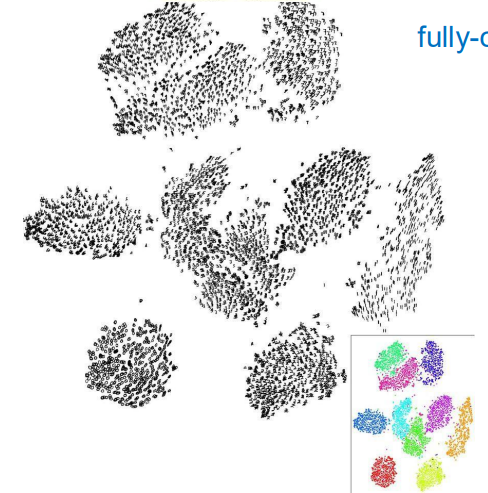
\includegraphics[width=0.5\linewidth]{img/lecture22/tsne ex.png}
    \caption{Figure 22.6: t-SNE visualization of MNIST}
    \label{fig:Exaample usage of TSNE}
\end{figure}


\subsection{Summary of Visualizing CNNs}

\subsubsection{Maximally Activating Patches}
Maximally activating patches correspond to regions of input images that produce the strongest responses in specific filters. This visualization helps reveal the types of visual patterns each neuron has learned to detect and provides insight into feature specialization within the network.

\subsubsection{Nearest Neighbor Images in Feature Space}
By examining images that lie closest to one another in the learned feature space, we can understand how the network groups visually and semantically similar inputs. This reveals how the CNN organizes images based on learned representations rather than raw pixel similarity.

\subsubsection{Last Layer Embeddings}
Visualizing last layer embeddings shows how images are positioned relative to each other in the high-level feature space. This perspective is useful for tasks such as clustering, image retrieval, and anomaly detection, and provides a global view of the network’s learned representation structure.

Together, these visualization techniques provide complementary insights into how CNNs learn hierarchical features, organize visual information, and make predictions.

\section{Saliency Methods}

Saliency methods aim to identify which regions of an input image are most important for a model’s prediction. One intuitive and widely used approach is \textbf{occlusion-based saliency}, which measures how the prediction changes when parts of the image are deliberately hidden. By observing how the model’s confidence varies as different regions are masked, we can infer which areas are most influential for the decision.

\subsection{Saliency via Occlusion}

Occlusion-based saliency generates heatmaps that visualize how blocking portions of an image affects the predicted class probabilities. For example, when key regions of an image containing an elephant are occluded, the model’s confidence in predicting the class ``elephant’’ drops significantly. This behavior reveals which spatial regions the network relies on most when forming its prediction.

This approach highlights the \textbf{network’s sensitivity} to specific visual regions. Rather than treating the image as a whole, the neural network focuses on particular structures that are strongly associated with the target class. The resulting heatmaps provide an intuitive and faithful explanation of the model’s decision-making process.

A major drawback of occlusion-based methods is their \textbf{computational cost}. To evaluate the importance of different regions, many occluded versions of the image must be processed by the network. For high-resolution images, this requires a large number of forward passes, making the method expensive in practice.

\subsubsection*{Connection to Feature Importance in Logistic Regression}

The intuition behind saliency maps is closely related to feature importance in linear models such as logistic regression:
\[
P(y = 1|x) = \sigma(\mathbf{w}^T x + b), \qquad 
P(y = 0|x) = 1 - \sigma(\mathbf{w}^T x + b)
\]

In logistic regression, each weight $w_i$ represents the importance of feature $x_i$ in determining the prediction. Large positive or negative weights indicate strong influence on the output probability. Similarly, saliency methods estimate how important each \emph{pixel region} is to the CNN’s prediction.

\begin{figure}[H]
    \centering
    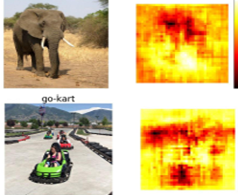
\includegraphics[width=0.5\linewidth]{img/lecture22/wi.png}
    \caption{Figure 22.7: Occlusion-based saliency heatmaps}
    \label{fig:Demonstartion}
\end{figure}


\subsection{Saliency via Gradients}

Gradient-based saliency provides a more efficient alternative to occlusion methods for estimating pixel importance. Instead of masking parts of the image repeatedly, we compute how sensitive the model’s prediction is to small changes in each input pixel. The resulting gradient-based saliency map highlights which pixels most strongly influence the output.

\subsubsection{Non-linear Mapping Function}

A deep neural network can be viewed as a highly non-linear function that maps an input image $x$ to a prediction $\hat{y}$ through multiple layers:

\[
\hat{y} = \phi \left( \cdots \phi \left( \phi \left( x \cdot w^{(1)} + b^{(1)} \right) \cdot w^{(2)} + b^{(2)} \right) \cdots \right)
\]

Here, $\phi$ represents activation functions (such as ReLU or sigmoid) that introduce non-linearity, while $w^{(i)}$ and $b^{(i)}$ denote the weights and biases of layer $i$. This composition of many non-linear transformations allows deep networks to model complex relationships between the input image and the predicted output.

\subsubsection{Linearization Using Taylor Approximation}

Although the full network is highly non-linear, we can understand its local behavior using a first-order Taylor approximation around a specific input:

\[
\hat{y} \approx \mathbf{w}^T x + b
\]

This approximation shows that, near a given input, the model behaves like a linear function. The gradient of the prediction with respect to the input,

\[
\nabla_x \hat{y} = \frac{\partial \hat{y}}{\partial x},
\]

measures how sensitive the prediction is to each input pixel. Pixels with large gradient magnitudes have the greatest influence on the output and are therefore considered most important.

A key advantage of gradient-based saliency is computational efficiency. Gradients can be computed using backpropagation in a single forward–backward pass, making the method practical even for high-dimensional images.

\begin{figure}[H]
    \centering
    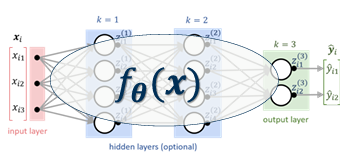
\includegraphics[width=0.4\linewidth]{img/lecture22/a.png}
    \caption{Figure 22.8: Highly non-linear mapping function}
    \label{Highly non-linear mapping function}
\end{figure}

\subsubsection{Computing Gradient-Based Saliency Maps}

We now illustrate how gradient-based saliency maps are generated in practice. The goal is to determine which pixels most influence the prediction for a chosen class.

\paragraph{Step 1: Forward Pass}

An input image is first passed through the neural network to compute class probabilities. For example, suppose the network outputs

\[
\hat{y} = \begin{bmatrix} 0.05 & 0.10 & 0.85 \end{bmatrix},
\]

where the highest probability corresponds to the class \textit{Dog}. This predicted class becomes the target for saliency analysis.

\begin{figure}[htbp]
    \centering
    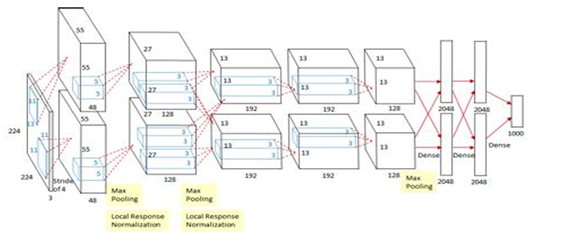
\includegraphics[width=0.8\linewidth]{img/lecture22/forward.png}
    \caption{Figure 22.9: Forward pass through the CNN}
    \label{fig:forward-pass}
\end{figure}

\paragraph{Step 2: Backward Pass}

Next, we compute the gradient of the selected class score with respect to the input image:

\[
\frac{\partial \hat{y}_{\text{dog}}}{\partial x}.
\]

This gradient measures how sensitive the predicted score is to small changes in each pixel. Pixels with large gradient magnitude have the strongest influence on the prediction.

In practice, this gradient is efficiently computed using backpropagation in a single backward pass through the network.

\paragraph{Step 3: Constructing the Saliency Map}

To visualize the importance of each pixel, we compute the maximum absolute gradient across the RGB channels. The resulting saliency map highlights image regions that most strongly affect the class score. Bright regions in the map correspond to pixels that are most critical for the network’s decision.

\paragraph{Example Interpretation}

Consider applying the gradient-based saliency procedure to several images from different classes. For each image, the network first predicts the most likely class and then computes the gradient of that class score with respect to the input pixels. The resulting saliency maps highlight the regions that most strongly influence the prediction.

For instance, in an image of a dog, the saliency map typically emphasizes the head, ears, and body contours rather than the background. Similarly, for objects such as boats or fruits, the highlighted regions correspond to the most distinctive visual features of the object. Across different examples, these maps consistently reveal that the network focuses on semantically meaningful structures rather than irrelevant background pixels.

This example interpretation demonstrates how gradient-based saliency provides an intuitive visual explanation of the model’s decision-making process.

\subsection{Saliency Methods: Weakly-Supervised Segmentation}

Saliency maps are not only useful for model interpretability but also serve as a practical tool for \textbf{weakly-supervised semantic segmentation}. In many real-world scenarios, obtaining pixel-level segmentation labels is expensive and time-consuming. Saliency maps provide an alternative by highlighting the regions of an image that most strongly influence the model’s prediction, offering a coarse localization of objects without requiring detailed annotations.

By computing gradients with respect to input pixels, the network identifies visually meaningful regions that correspond to objects or regions of interest. These highlighted regions can then be used as pseudo-labels to guide segmentation algorithms. Although the resulting segmentations may be coarse, they significantly reduce the need for fully labeled training data.

The visualizations below demonstrate how saliency-based segmentation reveals the network’s focus on different objects within an image, such as animals or foreground objects, while suppressing irrelevant background regions.

\begin{figure}[H]
  \centering
  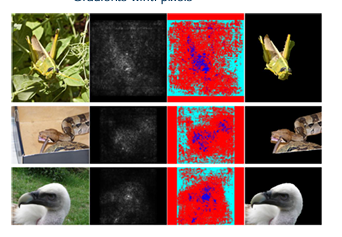
\includegraphics[width=0.8\textwidth]{img/lecture22/Picture3.png} 
  \caption{Figure 22.10: Examples of weakly-supervised segmentation using saliency maps.}
\end{figure}

\subsection{Uncovering Biases}

Saliency maps are not only useful for understanding \emph{how} a neural network makes a prediction, but also for diagnosing \emph{why it may fail}. In practice, deep models often learn spurious correlations present in the training data instead of the true semantic concepts we intend them to learn. Saliency visualization provides a powerful tool for uncovering these hidden biases by revealing which pixels most strongly influence a model’s decision.

A classic example involves training a classifier to distinguish wolves from dogs. Suppose that many wolf images in the training dataset contain snow in the background, while most dog images do not. Instead of learning the visual characteristics of wolves (such as facial structure or fur patterns), the model may learn that \emph{snow is a strong indicator of the “wolf” class}. As a result, when the network encounters an image of a husky standing in snow, it may confidently misclassify the dog as a wolf.

Figure~\ref{fig:wolf} shows an example of such a failure case. The model predicts the class \emph{wolf} for a husky image. However, the corresponding saliency map in Figure~\ref{fig:salient} reveals that the highest gradient magnitudes are concentrated on the snowy background rather than the animal itself. This indicates that the model is relying on contextual background cues instead of the object of interest. In other words, the classifier has unintentionally become a \emph{snow vs.\ no-snow classifier} rather than a true wolf vs.\ dog classifier.

This example highlights an important role of explainability methods in machine learning: they help practitioners detect dataset bias, diagnose model weaknesses, and guide improvements in data collection and model design. By revealing when a model is focusing on the wrong features, saliency methods provide actionable insights for building more robust and trustworthy systems.

\begin{figure}[H]
  \centering
  \begin{minipage}{0.45\textwidth}
    \centering
    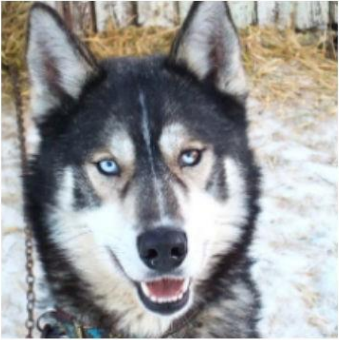
\includegraphics[width=\linewidth]{img/lecture22/wolf.png}
    \caption{Husky image misclassified as a wolf.}
    \label{fig:wolf}
  \end{minipage}
  \hfill
  \begin{minipage}{0.45\textwidth}
    \centering
    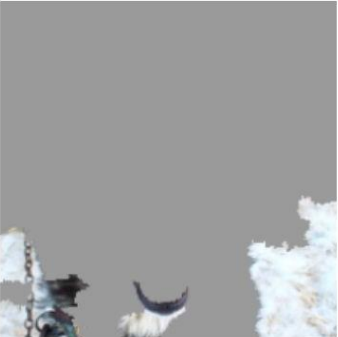
\includegraphics[width=\linewidth]{img/lecture22/salient.png}
    \caption{Saliency map highlighting snow as the dominant feature.}
    \label{fig:salient}
  \end{minipage}
\end{figure}

\section{Gradient-Based Explanations}

Gradient-based explanations provide insights into neural network decisions by identifying which parts of the input image most influence the model’s output. These methods rely on gradients computed during backpropagation to estimate how sensitive the prediction is to each input pixel. The resulting saliency maps visually highlight regions that strongly affect the output score.

A key advantage of gradient-based methods is their computational efficiency. Unlike occlusion-based approaches, which require repeatedly evaluating the model on modified inputs, gradients can be computed in a single backward pass. However, these explanations are only a local linear approximation of a highly non-linear model and therefore may not perfectly reflect the true decision-making process. In addition, raw gradients can sometimes lack class discriminativity and may highlight edges or textures that are not uniquely associated with the predicted class.

\subsection{Vanilla Backpropagation}

Vanilla backpropagation is the most direct approach for generating saliency maps. Given an input image and a target class score, we compute the gradient of the score with respect to the input pixels. The magnitude of this gradient indicates how strongly small changes in each pixel would affect the prediction.

In practice, the resulting saliency maps can be noisy and difficult to interpret. One reason is the presence of non-linear activation functions such as ReLU. During the backward pass, gradients are propagated only through neurons with positive activations, while negative activations are suppressed. This selective propagation emphasizes features that positively contribute to the prediction, helping highlight regions that are most relevant to the model’s decision.

Although simple, vanilla backpropagation forms the foundation for many improved gradient-based visualization techniques that aim to produce clearer and more stable explanations.

\subsection{Deconvnet Backpropagation}

Deconvnet backpropagation is a modified gradient-based visualization method designed to produce clearer and more interpretable saliency maps than vanilla backpropagation. The key idea is to change how gradients are propagated through ReLU non-linearities during the backward pass.

\subsubsection{Handling ReLU Non-linearities}

Recall that in the forward pass of a ReLU layer,
\[
h^{l+1} = \max(0, h^l).
\]
In standard backpropagation, gradients are propagated through ReLU units based on whether the *forward activation* was positive. Deconvnet modifies this rule by allowing gradients to flow only through neurons that have positive activations, effectively suppressing contributions from inactive regions.

\subsubsection{Backward Pass and Mathematical Formulation}

During the backward pass, the gradient propagation rule becomes
\[
\Delta h^l = \mathbf{1}(h^l > 0)\,\Delta h^{l+1},
\]
where the indicator function \(\mathbf{1}(h^l > 0)\) ensures that gradients are zeroed out whenever the forward activation is negative. This rectification removes noisy gradient signals and focuses the visualization on features that positively contribute to the prediction.

\subsubsection{Interpretation and Intuition}

By restricting gradient flow to regions with positive activations, deconvnet backpropagation produces sharper and more localized saliency maps than vanilla backpropagation. In practice, this leads to clearer highlighting of edges, textures, and object parts that strongly activate the network. The reduction in noise makes the resulting explanations easier to interpret, representing an important step toward more refined gradient-based explanation techniques.


\subsection{Forward and Backward Pass Details}

Figure~\ref{fig:ReLU Activation Forward and Backward Pass Illustration} illustrates how ReLU nonlinearities affect both the forward and backward passes of a neural network. Understanding this behavior is essential for interpreting gradient-based saliency methods, since these methods rely directly on the gradients propagated through the network.

\begin{figure}[H]
    \centering
    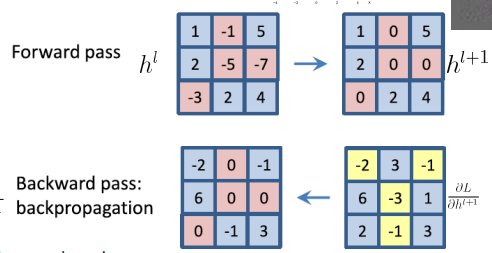
\includegraphics[width=0.5\linewidth]{img/lecture22/Details.png}
    \caption{Figure 22.12: ReLU activation in the forward and backward pass.}
    \label{fig:ReLU Activation Forward and Backward Pass Illustration}
\end{figure}

\subsubsection{ReLU Nonlinearities and Backpropagation}

During the forward pass, the ReLU activation function performs a simple element-wise operation that sets all negative activations to zero:
\[
h^{l+1} = \max(0, h^l).
\]
This operation introduces sparsity in the activations and allows the network to model non-linear relationships.

During the backward pass, this nonlinearity plays an equally important role in determining how gradients flow through the network. Because ReLU outputs zero for negative inputs, gradients are propagated only through neurons that were active during the forward pass. Mathematically, the gradient with respect to the previous layer is given by
\[
\frac{\partial L}{\partial h^l}
= \mathbf{1}[h^l > 0] \cdot \frac{\partial L}{\partial h^{l+1}},
\]
where the indicator function $\mathbf{1}[h^l > 0]$ blocks gradients at locations where the forward activation was negative. As a result, neurons that were inactive during the forward pass receive no gradient signal during backpropagation.

This gating behavior is crucial for saliency methods because it determines which spatial regions of the image can influence the gradient signal used to generate saliency maps.

\subsubsection{Deconvnet Backpropagation}

Deconvnet backpropagation modifies the standard backward pass by further restricting gradient flow. In addition to the forward-pass gating described above, this method propagates only *positive gradients* from the higher layer. Intuitively, this rectification step emphasizes features that positively contribute to the activation of the target class while suppressing noisy or irrelevant signals.

Formally, gradient propagation for layer $l$ can be written as
\[
\frac{\partial L}{\partial h^l}
= \mathbf{1}[h^l > 0] \cdot \frac{\partial L}{\partial h^{l+1}},
\]
with the additional constraint that only positive gradient values from the later layer are allowed to pass. This modification leads to sharper and more interpretable visualizations.

In practice, the combination of forward-pass gating and gradient rectification produces saliency maps that are significantly cleaner than those obtained with vanilla backpropagation. The resulting visualizations better highlight edges, textures, and object parts that strongly influence the network’s predictions.

\subsection{Guided Backpropagation}

Guided backpropagation further refines gradient-based saliency by combining the ideas of standard backpropagation and Deconvnet backpropagation. Recall that standard backpropagation allows gradients to pass only through neurons that were active during the forward pass, while Deconvnet backpropagation additionally restricts gradients to be positive. Guided backpropagation merges both constraints, allowing gradients to flow only when **both the forward activation and the backward gradient are positive**.

During the forward pass, the ReLU activation behaves as usual:
\[
h^{l+1} = \max\{0, h^l\}.
\]
However, during the backward pass, the gradient propagation rule becomes more restrictive:
\[
\frac{\partial L}{\partial h^l}
= \mathbf{1}[h^l > 0]\;
  \mathbf{1}\!\left[\frac{\partial L}{\partial h^{l+1}} > 0\right]
  \frac{\partial L}{\partial h^{l+1}}.
\]

This equation shows that gradient signals are allowed to pass only when two conditions are satisfied:
\begin{itemize}
\item The neuron was positively activated during the forward pass.
\item The gradient coming from the higher layer is positive.
\end{itemize}

By enforcing both constraints simultaneously, guided backpropagation suppresses noisy gradient signals and emphasizes features that positively contribute to the target class. In practice, this produces sharper and more visually interpretable saliency maps than either vanilla backpropagation or Deconvnet backpropagation. The resulting visualizations often highlight fine-grained structures such as edges, textures, and object boundaries, making guided backpropagation one of the most widely used gradient-based explanation techniques.


\subsection{Vanilla vs.\ Deconvnet vs.\ Guided Backpropagation}

The three gradient-based visualization methods discussed so far differ primarily in how they handle gradient flow through ReLU nonlinearities during the backward pass. These differences directly affect the quality and interpretability of the resulting saliency maps.

\textbf{Vanilla backpropagation} allows gradients to pass through ReLU units only when the corresponding neuron was active during the forward pass. Although this produces useful feature-importance maps, the resulting visualizations are often noisy and diffuse, making it difficult to clearly identify the most important image regions.

\textbf{Deconvnet backpropagation} improves upon this by additionally restricting gradients to be positive during the backward pass. This suppresses many irrelevant signals and produces sharper and more localized saliency maps that better highlight edges, textures, and object parts.

\textbf{Guided backpropagation} combines both constraints: gradients are allowed to flow only when the forward activation is positive \emph{and} the backward gradient is positive. This dual rectification removes a large portion of the noise present in earlier methods, typically producing the cleanest and most visually interpretable saliency maps among the three approaches.

Overall, these methods illustrate how small changes in gradient propagation rules can significantly improve the clarity of neural network explanations.

\subsection{Problems with Guided Backpropagation}

Although guided backpropagation produces visually appealing and sharp saliency maps, it has several important limitations. In particular, the method often lacks \textbf{class discriminativity} and may highlight image structures that are not truly responsible for the model’s prediction.

\paragraph{Issue 1: Lack of class discriminativity}

A key limitation is that guided backpropagation does not reliably distinguish between different output classes. In practice, saliency maps generated for different classes can appear surprisingly similar, even when the predicted categories are very different.

For example, consider generating guided backpropagation maps for the classes \emph{``airliner''} and \emph{``bus''}. Ideally, the explanation for each class should highlight class-specific features such as wings for airplanes or wheels and windows for buses. However, guided backpropagation often highlights generic edges, textures, and contours that appear in both images. This suggests that the method is emphasizing low-level image structure rather than class-specific semantic features.

This observation indicates that guided backpropagation is not always tightly coupled to the network’s final decision-making process. Instead, it often behaves like a generic edge detector influenced by the network’s learned filters.

\paragraph{Issue 2: Noise and ambiguity in class-specific saliency}

Another limitation is that gradient-based saliency maps can still be noisy and difficult to interpret. Even when guided backpropagation improves visual sharpness, it may fail to clearly differentiate between similar classes.

Consider saliency maps generated for images of a \emph{cat} and a \emph{dog}. Vanilla backpropagation typically produces noisy maps that highlight many irrelevant regions. Guided backpropagation reduces some of this noise, but the resulting maps may still highlight similar edges and textures in both images. As a result, the explanations may not clearly indicate why the network prefers one class over another.

Figure~\ref{fig:Example of backdrop} illustrates this phenomenon: saliency maps for different classes often look visually similar, revealing that the method does not strongly encode class-specific reasoning.

These limitations motivate the development of more advanced techniques (such as Grad-CAM) that explicitly incorporate class information when generating explanations.

 \begin{figure}[H]
     \centering
     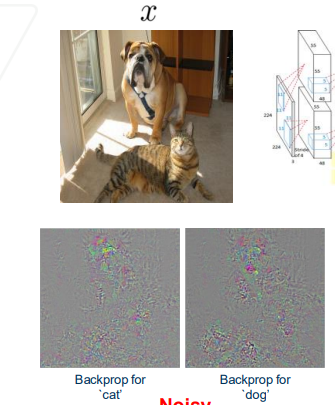
\includegraphics[width=0.3\linewidth]{img/lecture22/xdog.png}
     \caption{Figure 22.13: Example of noisy gradient-based saliency maps.}
     \label{fig:Example of backdrop}
 \end{figure}

\subsection{Summary of Saliency Maps}

Saliency methods can be broadly divided into two categories: \emph{intervention-based} methods and \emph{gradient-based} methods. Although both aim to identify which parts of an input most influence a model’s prediction, they differ significantly in methodology and computational cost.

\subsubsection{Intervention-Based Methods}

Intervention-based methods estimate feature importance by explicitly perturbing pixels (or regions) of the input and observing how the model’s output changes. By measuring the impact of each modification, these approaches provide an intuitive and often reliable estimate of which regions are critical for prediction.

However, this direct strategy comes with substantial drawbacks. Because each perturbation requires a separate forward pass through the network, these methods are computationally expensive. In practice, generating high-resolution saliency maps may require many iterative perturbations, making them slow and difficult to scale.

\subsubsection*{Gradient-Based Methods}

Gradient-based methods take a different approach by approximating feature importance using backpropagation. Instead of repeatedly modifying the input, these methods compute the gradient of the output with respect to the input in a single backward pass. This makes them significantly more computationally efficient than intervention-based approaches.

While gradient-based methods are fast and easy to implement, they rely on local linear approximations and may suffer from noise or lack of class discriminativity. Nevertheless, their efficiency and simplicity make them widely used in practice, especially for large-scale models.

Overall, the trade-off between intervention-based and gradient-based saliency methods reflects a broader theme in explainability: accuracy and interpretability often come at the cost of computational efficiency.

\section{Gradient-Based Class Activation Map (Grad-CAM)}

\subsection{Motivation}

Pixel-level saliency maps highlight regions that influence a prediction, but
they often suffer from noise and poor class discriminativity. Grad-CAM was
introduced to produce \emph{class-specific} visual explanations that are both
interpretable and spatially meaningful.

The objective of Grad-CAM is to identify which internal feature maps in a
convolutional neural network are most responsible for predicting a particular
class. For these explanations to be useful, the resulting activations must
satisfy two key requirements. First, they must be \textbf{class-discriminative},
meaning that the highlighted regions directly reflect the network’s reasoning
for a chosen class. Second, they must \textbf{preserve spatial information}, so
that the explanation can be mapped back onto the original image and interpreted
visually.

A key design decision is the choice of network layer to analyze. Early
convolutional layers retain high spatial resolution but capture only low-level
features such as edges and textures. Fully connected layers capture high-level
semantics but discard spatial structure. The \textbf{last convolutional layer}
provides the ideal compromise: it encodes rich semantic information while still
maintaining coarse spatial structure. Grad-CAM therefore operates on this layer
to produce meaningful localization maps.

\subsection{Method}

Grad-CAM computes a class-specific heatmap by combining feature maps using
weights derived from gradients of the target class score.

\begin{enumerate}
  \item \textbf{Forward Pass}
  \begin{itemize}
    \item Input an image into the CNN.
    \item Extract feature maps $A^k$ from the last convolutional layer.
    \item Compute the class score $y^c$ (logit) for the target class $c$.
  \end{itemize}

  \item \textbf{Backward Pass (Class-Specific Gradients)}
  \begin{itemize}
    \item Backpropagate gradients from the class score $y^c$ to the last
    convolutional layer.
    \item Compute importance weights for each feature map:
    \[
    \alpha_k^c = \frac{1}{Z}\sum_i\sum_j
    \frac{\partial y^c}{\partial A_{ij}^k},
    \]
    where $Z$ is the number of spatial locations.
  \end{itemize}

  \item \textbf{Compute the Class Activation Map}
  \[
  L_{\text{Grad-CAM}}^c =
  \mathrm{ReLU}\left(\sum_k \alpha_k^c A^k\right).
  \]
  This produces a coarse heatmap highlighting regions that positively influence
  the class prediction.

  \item \textbf{Visualization}
  \begin{itemize}
    \item Upsample the heatmap to the input image resolution.
    \item Overlay the heatmap on the original image.
  \end{itemize}
\end{enumerate}

\begin{figure}[H]
    \centering
    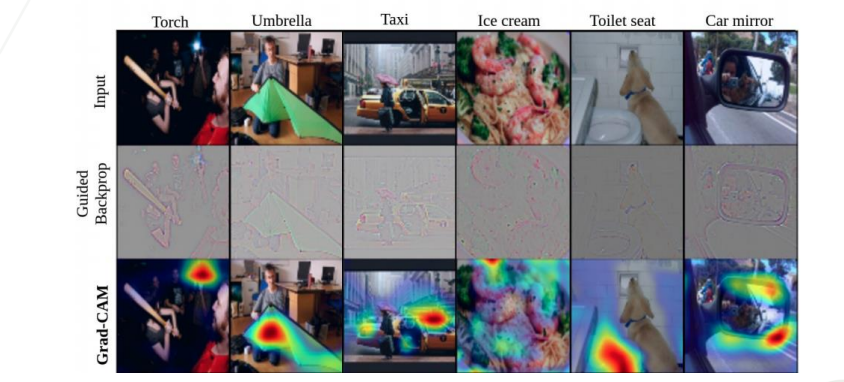
\includegraphics[width=0.75\linewidth]{img/lecture22/activation.png}
    \caption{Figure 22.14: Grad-CAM produces class-discriminative localization maps that
    highlight semantic regions responsible for the prediction.}
    \label{fig:gradcam_overview_l22}
\end{figure}

\begin{figure}[H]
    \centering
    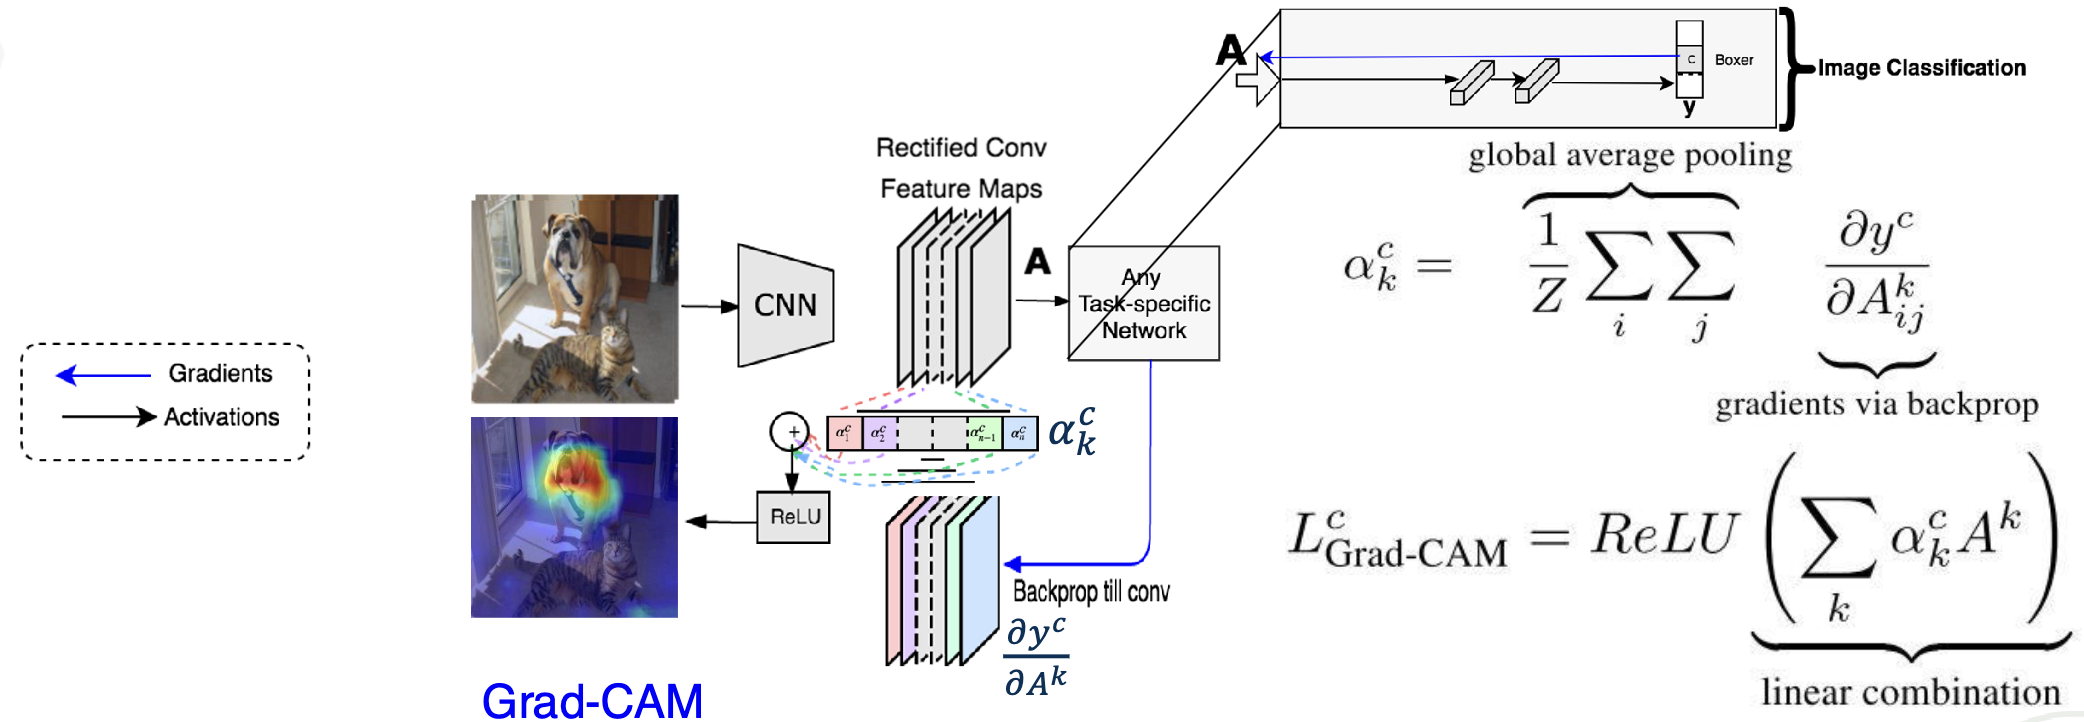
\includegraphics[width=0.8\linewidth]{img/lecture23/net15.png}
    \caption{Figure 22.15: Grad-CAM computation pipeline: forward pass, gradient
    backpropagation, global-average pooling of gradients, and weighted
    combination of feature maps.}
    \label{fig:gradcam_process_l22}
\end{figure}

Together, these steps allow Grad-CAM to connect internal feature representations
to human-interpretable image regions. Compared to Guided Backpropagation, which
often highlights edges and textures, Grad-CAM focuses on high-level semantic
regions responsible for the prediction.

\subsection{Interpretation and Practical Insights}

Grad-CAM provides clearer and more class-discriminative explanations than
gradient-only saliency methods. In practice, Guided Backpropagation often
highlights fine edges and textures throughout the image, including background
details that are not directly responsible for the model’s prediction. 

Grad-CAM, in contrast, focuses on \textbf{semantic regions} that contribute most
strongly to the predicted class. This difference makes Grad-CAM particularly
useful for understanding \emph{where} the network is looking when making a
decision, rather than simply which pixels produce large gradients.

This property makes Grad-CAM an effective tool for debugging models, detecting
failure modes, and building trust in neural network predictions.

% % TODO: MOVE TO Lecture 23
% \section{Key Questions in Explainability}

% Explainability methods are ultimately designed to answer different types of
% questions about model behavior. Understanding these question types helps
% clarify why different explanation techniques exist.

% \textbf{Correlational Questions — “Why P?”}  
% These questions identify which input features are associated with a prediction.
% Methods such as saliency maps and Grad-CAM fall into this category because they
% highlight regions that correlate with the predicted class.

% \textbf{Counterfactual Questions — “What if?”}  
% These questions explore how predictions would change if the input were modified.
% Counterfactual explanations test model robustness and sensitivity by asking how
% small changes in the input could alter the prediction.

% \textbf{Contrastive Questions — “Why P rather than Q?”}  
% These questions focus on discriminative reasoning. Instead of explaining why a
% prediction occurred, they explain why one class was chosen instead of another.
% Contrastive explanations are especially useful in fine-grained recognition tasks
% where classes share similar visual features.

% These three question types form the conceptual foundation for more advanced
% explanation methods introduced next.


% % TODO: MOVE TO Lecture 23
% \section{Types of Explanations}

% Explainability methods can be grouped into three broad categories based on how
% directly they relate explanations to the model’s decision.

% \subsection{Indirect Explanations}

% Indirect explanations analyze internal network components such as weights,
% feature maps, or neuron activations. These methods expose intermediate
% representations and are most useful for expert users who want to understand how
% the model processes information internally.

% \subsection{Direct Explanations}

% Direct explanations operate in the input space and highlight which regions of
% the input most influence the prediction. Saliency maps and Grad-CAM are common
% examples because they visually show which image regions contribute to the
% model’s decision.

% \subsection{Targeted Explanations}

% Targeted explanations focus on explaining a specific prediction. Rather than
% producing a general importance map, they answer targeted questions such as
% “Why this class?” or “Why this class instead of another?”. These methods build
% on the question types introduced earlier and motivate more advanced approaches
% such as contrastive and counterfactual explanations.


% % TODO: Move to lecture 23
% \section{Targeted Explanation Methods}

% We now introduce explanation methods designed to answer the 
% \textbf{contrastive} and \textbf{counterfactual} questions introduced earlier.  
% Unlike general saliency maps that ask \textit{Why this prediction?}, targeted
% explanations aim to answer more specific questions about model decisions.

% \begin{figure}[H]
%     \centering
%     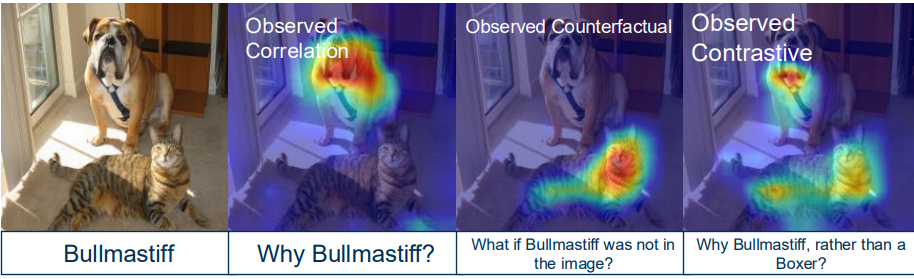
\includegraphics[width=0.7\linewidth]{img/lecture22/target.png}
%     \caption{Types of Saliency Maps for Dog Image Classification}
% \end{figure}

% The figure above illustrates how different explanation paradigms correspond to
% different question types: correlational (Why this?), counterfactual (What if?),
% and contrastive (Why this rather than that?).

% \subsection{\textbf{Contrast-CAM}}

% \textbf{Contrast-CAM} explains why the model predicts one class instead of
% another. Rather than asking \textit{Why this class?}, it asks:

% \begin{center}
% \textit{Why class $P$ rather than class $Q$?}
% \end{center}

% By comparing gradients from competing classes, Contrast-CAM highlights the
% image regions that support one prediction while suppressing evidence for the
% alternative class. This makes it particularly useful for fine-grained
% classification problems where multiple classes share similar visual features.

% \subsection{\textbf{Counterfactual-CAM}}

% \textbf{Counterfactual-CAM} explores how explanations would change if the model
% predicted a different class. This answers the question:

% \begin{center}
% \textit{What would need to change for the prediction to be different?}
% \end{center}

% By visualizing activation maps under alternative class assumptions, this method
% reveals which features the model relies on and how sensitive the prediction is
% to input changes.

% \subsection{Relationship to Grad-CAM}

% Together, \textbf{Grad-CAM}, \textbf{Contrast-CAM}, and
% \textbf{Counterfactual-CAM} form a family of \textbf{targeted explanation
% techniques}. These methods move beyond generic saliency maps by explicitly
% connecting explanations to specific question types about model behavior.

% For completeness, recall that Grad-CAM computes feature-map importance weights
% by averaging gradients of the class score with respect to feature-map
% activations:
% \[
% \alpha_k^c = \frac{1}{Z}\sum_i\sum_j
% \frac{\partial y^c}{\partial A_{ij}^k}.
% \]

% The class activation map is then computed as:
% \[
% L_{\text{Grad-CAM}}^c
% = \mathrm{ReLU}\!\left(\sum_k \alpha_k^c A^k\right).
% \]

% This produces a spatial heatmap highlighting the regions that positively
% influence the target class prediction.


% \section{Evaluating Explanations}

% Producing visually appealing explanations is not sufficient. We must evaluate
% whether explanations (i) faithfully reflect the model's decision process and
% (ii) are useful to humans in practice. Evaluation therefore combines
% \textbf{quantitative (automated)} tests with \textbf{human-centered} studies.

% \subsection{Evaluation Criteria}

% In practice, explanation quality is often judged along three complementary axes:

% \begin{itemize}
%     \item \textbf{Human interpretability:} Are the explanations understandable to non-experts, and do they help users build appropriate trust in model predictions?
%     \item \textbf{Model transparency:} Do the explanations reveal meaningful insights about what the model is using internally to make decisions, supporting validation and reliability?
%     \item \textbf{Operational usability:} Can the explanations be used to debug models, diagnose failure modes or bias, and guide model refinement?
% \end{itemize}

% The methods below provide concrete ways to measure these criteria.

% \subsection{Quantitative Evaluation via Masking}

% A widely used automated evaluation strategy is \textbf{masking}. Explanation
% heatmaps are used as masks to modify the input and observe how the model's
% confidence changes. The intuition is simple:

% \begin{center}
% \textit{If an explanation correctly identifies important pixels, removing those
% pixels should strongly damage the prediction, while keeping only those pixels
% should preserve it.}
% \end{center}

% Masking techniques therefore provide a quantitative way to test whether an
% explanation reflects the model's decision process.

% \subsubsection{Heatmap Masking}

% This approach uses the entire explanation heatmap to determine which regions of
% the image to obscure. Typically, the highest-importance regions are progressively
% removed, and the resulting change in prediction confidence is measured. A rapid
% drop in confidence indicates that the explanation identified regions that are
% important to the model.

% \subsubsection{Pixel-wise Importance Masking}

% Instead of masking contiguous regions, pixels are removed (or retained)
% individually in order of importance. By tracking how confidence changes as pixels
% are removed or inserted, we obtain a finer-grained evaluation of the model's
% dependency on specific visual features.

% \subsection{Insertion and Deletion Metrics}

% A standard quantitative benchmark for explainability is
% \textbf{progressive pixel-wise insertion and deletion}. This method measures how
% model confidence changes as pixels are gradually removed or revealed according
% to their importance scores.

% \paragraph{Pixel-wise Deletion}
% Pixels are sequentially removed from most to least important. If the explanation
% is accurate, the model's confidence in the correct class should drop rapidly as
% the most informative pixels are deleted.

% \paragraph{Pixel-wise Insertion}
% Starting from a blurred or empty image, pixels are added back in order of
% importance. A faithful explanation causes the model's confidence to increase
% quickly as informative pixels are inserted.

% \subsection{Human-Centered Evaluation}

% While quantitative metrics provide important benchmarks, the ultimate goal of
% explainability is to help humans understand and trust model decisions. For this
% reason, explanation methods are also evaluated using human judgment and
% perception.

% \subsubsection{Gaze Tracking}

% Gaze tracking measures where individuals focus their visual attention when
% interpreting an explanation. By comparing eye-fixation patterns with explanation
% heatmaps, researchers can assess whether model explanations align with natural
% human perception and visual reasoning. Strong alignment suggests that the model
% highlights regions that humans also consider informative.

% \subsubsection{Pointing Games}

% In pointing games, users are asked to indicate which regions of an explanation
% they find most informative for a prediction. Agreement between human-selected
% regions and explanation maps provides evidence that the model highlights
% features that humans consider meaningful and relevant for the task.

% \subsubsection{User Studies and Comparative Evaluation}

% User studies compare different explanation techniques and ask participants to
% rate clarity, usefulness, and trustworthiness. Comparative studies can also
% present multiple explanation methods side-by-side (for example, vanilla
% Backpropagation, Deconvolution, and Guided Backpropagation) and evaluate user
% preference, perceived clarity, and alignment with expected reasoning patterns.

% \begin{figure}[H]
%     \centering
%     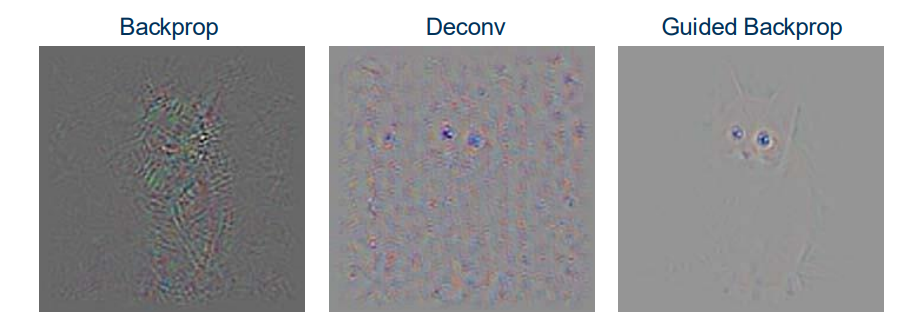
\includegraphics[width=0.5\linewidth]{img/lecture22/aa.png}
%     \caption{Human evaluation of gradient-based visualization methods.}
%     \label{fig:Human Evaluation}
% \end{figure}

% Figure~\ref{fig:Human Evaluation} demonstrates that different gradient-based
% visualization techniques can vary substantially in interpretability when judged
% by humans, motivating comparative evaluation protocols.

% \begin{figure}[H]
%     \centering
%     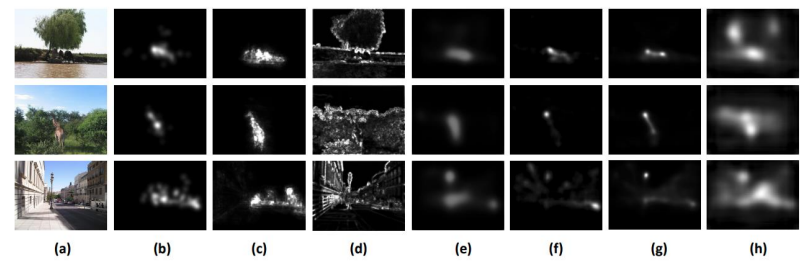
\includegraphics[width=0.5\linewidth]{img/lecture22/vsi.png}
%     \caption{Saliency maps compared across explanation methods.}
%     \label{fig:Saliency Map Visualization}
% \end{figure}

% Figure~\ref{fig:Saliency Map Visualization} provides a side-by-side comparison
% of saliency maps generated by multiple explanation and saliency detection
% methods applied to the same input images. The subfigures correspond to:
% \begin{itemize}
%     \item (a) Input image
%     \item (b) Human ground-truth fixation map
%     \item (c) Proposed implicit saliency method
%     \item (d) Feed-forward feature saliency
%     \item (e) SalGAN
%     \item (f) ML-Net
%     \item (g) DeepGaze II
%     \item (h) ShallowDeep
% \end{itemize}
% Comparing these maps allows researchers to evaluate how closely different
% methods align with human visual attention. Methods that consistently highlight
% semantically meaningful regions and resemble human fixation maps are considered
% more human-aligned explanations.

% Together, automated and human-centered evaluation provide a comprehensive
% framework for assessing explanation quality.

% \section{Visual Aids}

% Throughout this lecture, a variety of visual aids are used to illustrate how explanation techniques reveal the internal behavior of neural networks. Feature importance maps provide an intuitive view of which regions of an input most strongly influence a model’s prediction, helping translate abstract gradients into human-interpretable patterns. 

% In addition, layer activation visualizations offer insight into how representations evolve across the network. By observing how different layers respond to the same input, we gain a deeper understanding of how low-level features develop into high-level semantic concepts. Together, these visual tools play a crucial role in making modern deep learning models more interpretable and accessible.

% \section{Targeted Explanations}

% \begin{figure}[H]
%     \centering
%     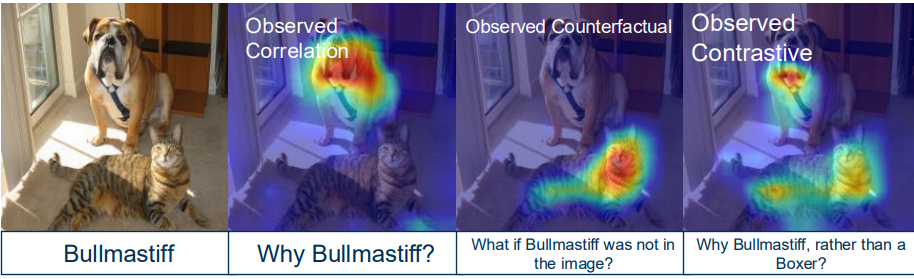
\includegraphics[width=0.7\linewidth]{img/lecture22/target.png}
%     \caption{Types of Saliency Maps for Dog Image Classification}
% \end{figure}

% \subsection{Contrast-CAM and Counterfactual-CAM}

% Beyond standard Grad-CAM, several extensions aim to provide \textit{targeted explanations} that answer more specific questions about model decisions. 

% \textbf{Contrast-CAM} focuses on comparing two competing classes by highlighting the regions that support one prediction over another. Rather than asking “Why this class?”, it asks “Why this class instead of another?”. This is especially useful for fine-grained recognition tasks where multiple classes share similar visual features.

% \textbf{Counterfactual-CAM} instead explores how the explanation would change if the model predicted a different class. By visualizing how activation maps shift under alternative predictions, this method reveals which features the model relies on and how sensitive the prediction is to changes in the input.

% \subsection*{Grad-CAM Formulation Revisited}

% The Grad-CAM method computes importance weights for each feature map by averaging the gradients of the class score with respect to the feature map activations:
% \[
% \alpha_k^c = \frac{1}{Z} \sum_i \sum_j 
% \frac{\partial y^c}{\partial A_{ij}^k}.
% \]
% These weights measure how strongly feature map $k$ contributes to the class score $y^c$.

% The final class activation map is obtained by combining the feature maps using these weights and applying a ReLU:
% \[
% L_{\text{Grad-CAM}}^c
% = \mathrm{ReLU}\!\left(\sum_k \alpha_k^c A^k\right).
% \]
% This step retains only regions that positively influence the class prediction, producing a spatial heatmap that highlights the most relevant image regions.

% \section{Overview of Explainability Techniques}

% Visualization techniques such as Grad-CAM (Gradient-weighted Class Activation Mapping) help reveal how different regions of an input image influence a neural network’s prediction. Grad-CAM generates heatmap visualizations that highlight the most influential areas of the image for a specific class, providing an intuitive way to inspect model behavior. Through case studies across different models and tasks, these visualizations demonstrate how explanation techniques improve the interpretability and transparency of complex neural networks.

% \section{Explanatory Evaluation}
% \subsection{Evaluation Metrics}

% Explanations should ultimately be evaluated based on how useful and meaningful they are in practice. 

% \textbf{Human interpretability} assesses whether the explanations are understandable to non-experts and help users build trust in model predictions. 

% \textbf{Model transparency} examines whether the explanations reveal insights about the model’s internal decision-making process, which is essential for validation and reliability. 

% \textbf{Operational usability} evaluates whether explanations can be used in practice to debug models, improve performance, or guide model refinement.

% \section{Network Evaluation}

% \subsection{Purpose and Methodology}

% Beyond generating visually appealing explanations, it is important to evaluate how explanation techniques influence the behavior and performance of neural networks. Network evaluation examines whether explanations faithfully reflect the model’s decision-making process and whether they can be used to validate predictions without requiring direct human intervention.

% One common evaluation strategy is \textbf{explanation masking}. In this approach, regions of the input image are masked according to their importance scores derived from explanation heatmaps. By progressively removing or retaining highly ranked pixels, we can observe how the model’s prediction confidence changes. If masking the most important regions significantly degrades performance, this suggests that the explanation correctly identified critical features. Conversely, if performance remains stable, the explanation may not accurately capture the model’s true reasoning process.

% \subsection{Application Evaluation}

% In addition to automated evaluation techniques, explanations can be assessed through \textbf{human-centric evaluation tasks}. These approaches incorporate human judgment into the evaluation loop, even when precise quantitative metrics for explainability are difficult to define.

% Two widely used methods are \textbf{gaze tracking} and \textbf{pointing games}. Gaze tracking measures where individuals focus their visual attention when interpreting an explanation, allowing researchers to determine whether explanation heatmaps align with natural human perception. Pointing games, in contrast, require users to indicate which regions of an explanation they find most informative. These methods help assess whether explanation maps correspond to intuitive human reasoning.

% \begin{figure}[H]
%     \centering
%     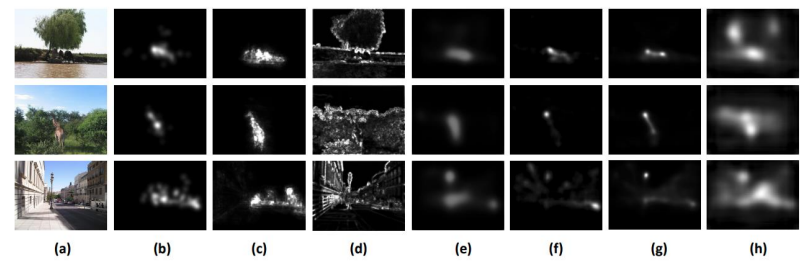
\includegraphics[width=0.5\linewidth]{img/lecture22/vsi.png}
%     \caption{Saliency Map Visualization}
%     \label{fig:Saliency Map Visualization}
% \end{figure}

% Figure~\ref{fig:Saliency Map Visualization} illustrates how saliency maps can be visually compared to evaluate whether highlighted regions align with meaningful image content.

% \subsection{Human Evaluation}

% Finally, explanations may be evaluated through \textbf{direct human interaction}. In this setting, participants are asked to assess the clarity, usefulness, and interpretability of explanations produced by AI systems. Such studies provide valuable insights into whether explanation methods truly assist users in understanding model decisions.

% Comparative studies are often conducted to determine which explanation techniques are most intuitive. For example, methods such as vanilla Backpropagation, Deconvolution, and Guided Backpropagation can be presented side by side and evaluated based on user preference, perceived clarity, and alignment with expected reasoning patterns.

% \begin{figure}[H]
%     \centering
%     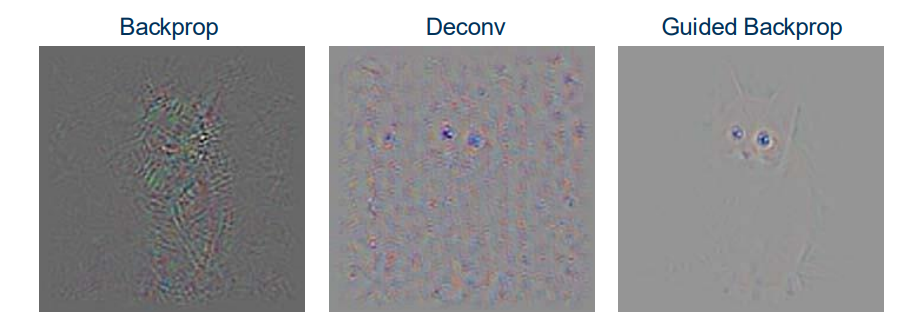
\includegraphics[width=0.5\linewidth]{img/lecture22/aa.png}
%     \caption{Human Evaluation}
%     \label{fig:Human Evaluation}
% \end{figure}

% Figure~\ref{fig:Human Evaluation} demonstrates how different gradient-based visualization methods may vary in interpretability when assessed by human observers.

% \section{Network Evaluation via Masking}

% Masking techniques provide a quantitative way to evaluate whether explanation maps accurately identify the regions that drive a model’s prediction. By selectively obscuring parts of the input image according to importance scores, we can measure how sensitive the model’s output is to those regions. If masking highly ranked regions significantly reduces prediction confidence, this suggests that the explanation correctly identified critical features.

% Two common masking strategies are used in practice.

% \textbf{Heatmap Masking.}  
% This approach uses the entire explanation heatmap to determine which regions to obscure. Typically, the highest-importance regions are progressively removed, and the resulting change in model confidence is measured. This method evaluates whether the explanation map, as a whole, captures meaningful predictive structure.

% \textbf{Pixel-wise Importance Masking.}  
% Instead of masking large contiguous regions, this approach removes pixels individually based on their importance scores. By observing how prediction confidence changes as individual pixels are removed or inserted, we can obtain a finer-grained assessment of the model’s dependency on specific image components.

% \section{Explanatory Evaluation}

% A widely used quantitative strategy for assessing explanation quality is 
% \textbf{progressive pixel-wise insertion and deletion}. These techniques evaluate whether the pixels identified as important by an explanation genuinely influence the model’s prediction.

% \textbf{Pixel-wise Deletion.}  
% In this procedure, pixels are systematically removed from the input image in order of decreasing importance. Importance scores are typically derived from the model’s sensitivity to each pixel’s contribution. The model’s prediction confidence is then tracked as information is removed. A rapid decline in confidence indicates that the explanation has successfully identified features that are critical to the model’s decision-making process.

% \textbf{Pixel-wise Insertion.}  
% The complementary procedure begins with a blank or heavily blurred image and gradually adds pixels back in order of importance. As informative pixels are inserted, the model’s prediction confidence should increase. This evaluates whether the highlighted features are sufficient to reconstruct the prediction and provides evidence that the explanation captures meaningful decision-making signals.

% \subsection{Additional Insights}

% These masking-based evaluations demonstrate the significant impact that the strategic removal or addition of pixels can have on model predictions. By controlling which parts of an image remain visible, researchers can directly test the robustness of a model and its dependence on specific visual features for classification and prediction tasks.

% Visual case studies further illustrate how different masking strategies can alter model outputs. These examples show how changes in the visibility of specific regions can lead to different predictions, highlighting the interpretive power of pixel-wise analysis. Such case studies also make it easier to communicate complex explainability concepts and demonstrate the practical value of explanation techniques in real-world applications.

\section{Q\&A Section}

\begin{enumerate}

\item \textbf{Question:}
Compare occlusion-based saliency and gradient-based saliency in terms of
faithfulness and computational cost.

\textbf{Solution:}
Occlusion-based saliency measures importance by directly perturbing the input
and observing changes in the prediction, making it causally grounded but
computationally expensive due to many forward passes.  
Gradient-based saliency is efficient (single forward/backward pass) but
provides only a local linear approximation of importance.

\item \textbf{Question:}
Explain why early convolutional layers and fully connected layers are both
unsuitable for producing meaningful localization maps in Grad-CAM.

\textbf{Solution:}
Early layers retain spatial resolution but encode only low-level features
(edges/textures), lacking semantic meaning.  
Fully connected layers capture high-level semantics but discard spatial
structure.  
Grad-CAM therefore uses the last convolutional layer as a compromise.

\item \textbf{Question:}
How do Vanilla Backpropagation, Deconvnet, and Guided Backpropagation differ
in how they handle gradients through ReLU?

\textbf{Solution:}
Vanilla BP blocks gradients where forward activations were negative.  
Deconvnet blocks negative gradients during the backward pass.  
Guided BP blocks gradients unless both the forward activation and backward
gradient are positive, producing sharper maps.

\item \textbf{Question:}
Why does Guided Backpropagation lack class discriminativity?

\textbf{Solution:}
It primarily highlights generic edges and textures based on gradient flow,
rather than weighting feature maps by class-specific importance.  
As a result, maps for different classes often appear similar.

\item \textbf{Question:}
In Grad-CAM, what is the interpretation of the weight
\[
\alpha_k^c = \frac{1}{Z} \sum_{i,j} \frac{\partial y^c}{\partial A_{ij}^k} ?
\]

\textbf{Solution:}
It measures how strongly feature map $k$ influences the target class score
$y^c$ on average across spatial locations.  
These weights determine how much each feature map contributes to the final
class activation map.

\item \textbf{Question:}
Why is a ReLU applied after computing
\[
L_{\text{Grad-CAM}}^c = \sum_k \alpha_k^c A^k ?
\]

\textbf{Solution:}
ReLU removes negative contributions, retaining only features that positively
support the target class.  
This improves interpretability by focusing the heatmap on regions that provide
evidence \emph{for} the class rather than against it.

\end{enumerate}

\end{document}
